\documentclass[a4paper,11pt]{report}

\usepackage{amsmath}
\usepackage{fullpage}
\usepackage{tikz}

\usetikzlibrary{graphs,graphs.standard}

\makeatletter
\pgfmathdeclarefunction{alpha}{1}{%
  \pgfmathint@{#1}%
  \edef\pgfmathresult{\pgffor@alpha{\pgfmathresult}}%
}

\usepackage{bussproofs}
\usepackage{mathpartir}
\usepackage{prooftrees}
\usepackage{color}

\newcommand*{\contract}[2]{contraction of $#1$ with $#2$}

\usepackage{tikz}
\usetikzlibrary{automata,positioning}

\author{Sylvain Julmy}
\date{\today}

\setlength{\parindent}{0pt}

\begin{document}

\begin{center}
  \Large{
    Mathematical Methods for Computer Science 2\
    Fall 2017
  }
  \noindent\makebox[\linewidth]{\rule{\linewidth}{0.4pt}}

  Series 7
  \vspace*{1.4cm}

  Sylvain Julmy
  
  \noindent\makebox[\linewidth]{\rule{\linewidth}{0.4pt}}
\end{center}

\section*{\texttt{1}}

\[
  q_0' = \{q_0\} = \{q_0,q_1,q_2\}
\]

\[
  \begin{array}{c|ccc}
    & a & b & c \\ \hline
    \{q_0,q_1,q_2\} & \{q_0\} & \{q_1,q_2\} & \{q_0,q_1,q_2\} \\
    \{q_0\} & \emptyset & \{q_1\} & \{q_2\} \\
    \{q_1,q_2\} & \{q_0\} & \{q_2\} & \{q_0,q_1\} \\
    \{q_0,q_1\} & \{q_0\} & \{q_1,q_2\} & \{q_0,q_1,q_2\} \\
    \{q_1\} & \{q_0\} & \{q_2\} & \{q_0,q_1\} \\
    \{q_2\} & \emptyset & \emptyset & \emptyset \\
    \emptyset & \emptyset & \emptyset & \emptyset \\
  \end{array}
\]


\begin{center}
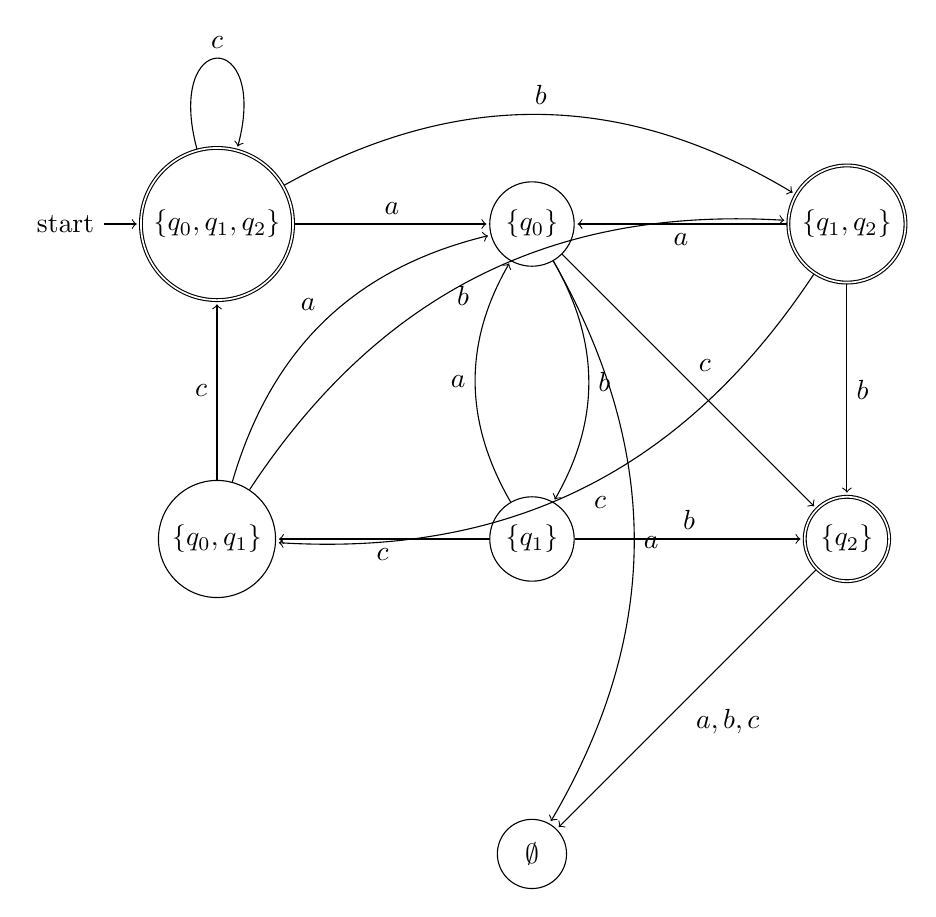
\begin{tikzpicture}[shorten >=1pt,node distance=4cm,on grid,auto]
  \node[state,initial,accepting] (q012) {$\{q_0,q_1,q_2\}$};
  \node[state] (q0) [right = of q012] {$\{q_0\}$};
  \node[state,accepting] (q12) [right = of q0] {$\{q_1,q_2\}$};
  \node[state] (q01) [below = of q012] {$\{q_0,q_1\}$};
  \node[state] (q1) [right = of q01] {$\{q_1\}$};
  \node[state,accepting] (q2) [right = of q1] {$\{q_2\}$};
  \node[state] (qe) [below = of q1] {$\emptyset$};
  \path[->]
  (q012)
  edge [] node [] {$a$} (q0)
  edge [bend left] node [] {$b$} (q12)
  edge [loop above] node [] {$c$} ()
  (q0)
  edge [bend left] node [] {$a$} (qe)
  edge [bend left] node [] {$b$} (q1)
  edge [] node [] {$c$} (q2)
  (q12)
  edge [] node [] {$a$} (q0)
  edge [] node [] {$b$} (q2)
  edge [bend left] node [] {$c$} (q01)
  (q01)
  edge [bend left] node [] {$a$} (q0)
  edge [bend left] node [below left] {$b$} (q12)
  edge [] node [] {$c$} (q012)
  (q1)
  edge [bend left] node [] {$a$} (q0)
  edge [] node [] {$b$} (q2)
  edge [] node [] {$c$} (q01)
  (q2)
  edge [] node [] {$a,b,c$} (qe)
  ;
\end{tikzpicture}
\end{center}

\section*{\texttt{2}}

No answer.

\section*{\texttt{3}}

We denote by $\Sigma^*$ any possible symbol from the alphabet.

\paragraph{DFA :}
\begin{center}
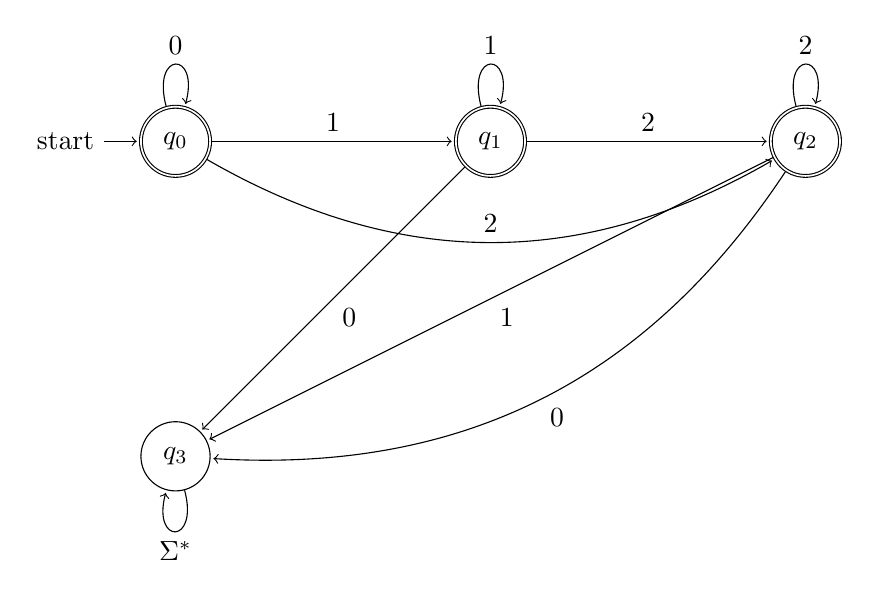
\begin{tikzpicture}[shorten >=1pt,node distance=4cm,on grid,auto]
  \node[state,initial,accepting] (q0) {$q_0$};
  \node[state,accepting] (q1) [right = of q0] {$q_1$};
  \node[state,accepting] (q2) [right = of q1] {$q_2$};
  \node[state] (q3) [below = of q0] {$q_3$};
  \path[->]
  (q0)
  edge [loop above] node [] {0} ()
  edge [] node [] {1} (q1)
  edge [bend right] node [] {2} (q2)
  (q1)
  edge [] node [] {0} (q3)
  edge [loop above] node [] {1} ()
  edge [] node [] {2} (q2)
  (q2)
  edge [loop above] node [] {2} ()
  edge [bend left] node [] {0} (q3)
  edge [] node [] {1} (q3)
  (q3)
  edge [loop below] node [] {$\Sigma^*$} ()
  ;
\end{tikzpicture}
\end{center}

\paragraph{$\epsilon$-NFA :}

\begin{center}
\begin{tikzpicture}[shorten >=1pt,node distance=4cm,on grid,auto]
  \node[state,initial] (q0) {$q_0$};
  \node[state,accepting] (q1) [right = of q0] {$q_1$};
  \node[state,accepting] (q2) [right = of q1] {$q_2$};
  \node[state] (q3) [below = of q1] {$q_3$};
  \path[->]
  (q0)
  edge [loop above] node [] {$0$} ()
  edge [] node [] {$\epsilon,1$} (q1)
  (q1)
  edge [loop above] node [] {$1$} ()
  edge [] node [] {$\epsilon,2$} (q2)
  edge [] node [] {$0$} (q3)
  (q2)
  edge [loop above] node [] {$2$} ()
  edge [] node [] {$0,1$} (q3)
  (q3)
  edge [loop below] node [] {$\Sigma^*$} ()
  ;
\end{tikzpicture}
\end{center}

\section*{\texttt{4}}

\subsection*{(a)}

\[
  (0 + 1)^*
  11
  (0 + 1)^*
\]

\subsection*{(b)}

\[
  (0+1)^* 0 (0+1)^* 0 (0+1)^*
\]

\subsection*{(c)}

\[
  1^* 0 1^* 0 1^*
\]

\subsection*{(d)}

\[
  (1^* 0 1^* 0 1^*)^*
\]

\section*{\texttt{5}}

\subsection*{(a)}

Any number (represented by the length of a word in a unary alphabet) which can
be represented by bill of $17$ and $31$. For example, $17 = 1 \cdot 17 + 0 \cdot
31$ or $ 175 = 3 \cdot 17 + 4 \cdot 31$.

\subsection*{(b)}

Any binary word of $0$ and $1$, including the empty word.

\subsection*{(c)}

The words of alternating sequence of $0$ and $1$ which ends by a $1$.

\end{document}
